%%
%% Automatically generated file from DocOnce source
%% (https://github.com/hplgit/doconce/)
%%
%%


%-------------------- begin preamble ----------------------

\documentclass[%
oneside,                 % oneside: electronic viewing, twoside: printing
final,                   % draft: marks overfull hboxes, figures with paths
10pt]{article}

\listfiles               %  print all files needed to compile this document
\usepackage{mathtools}
\usepackage{relsize,makeidx,color,setspace,amsmath,amsfonts,amssymb}
\usepackage[table]{xcolor}
\usepackage{bm,ltablex,microtype}
\usepackage{float}
\usepackage[pdftex]{graphicx}
\usepackage{epstopdf}
\usepackage{verbatim}

\usepackage{fancyvrb} % packages needed for verbatim environments

\usepackage[T1]{fontenc}
%\usepackage[latin1]{inputenc}
\usepackage{ucs}
\usepackage[utf8x]{inputenc}
\usepackage[english]{babel}
\usepackage{lmodern}         % Latin Modern fonts derived from Computer Modern

% Hyperlinks in PDF:
\definecolor{linkcolor}{rgb}{0,0,0.4}
\usepackage{hyperref}
\hypersetup{
    breaklinks=true,
    colorlinks=true,
    linkcolor=linkcolor,
    urlcolor=linkcolor,
    citecolor=black,
    filecolor=black,
    %filecolor=blue,
    pdfmenubar=true,
    pdftoolbar=true,
    bookmarksdepth=3   % Uncomment (and tweak) for PDF bookmarks with more levels than the TOC
    }
%\hyperbaseurl{}   % hyperlinks are relative to this root

\setcounter{tocdepth}{2}  % levels in table of contents



% prevent orhpans and widows
\clubpenalty = 10000
\widowpenalty = 10000

% --- end of standard preamble for documents ---


% insert custom LaTeX commands...

\raggedbottom
\makeindex
\usepackage[totoc]{idxlayout}   % for index in the toc
\usepackage[nottoc]{tocbibind}  % for references/bibliography in the toc

%-------------------- end preamble ----------------------

\begin{document}

% matching end for #ifdef PREAMBLE

\newcommand{\exercisesection}[1]{\subsection*{#1}}


% ------------------- main content ----------------------



% ----------------- title -------------------------

\thispagestyle{empty}

\begin{center}
{\LARGE\bf
\begin{spacing}{1.25}
PHYS 905 - Project 3
\end{spacing}
}
\end{center}

% ----------------- author(s) -------------------------

\begin{center}
{\bf Terri Poxon-Pearson}
\end{center}

    
% ----------------- end author(s) -------------------------

% --- begin date ---
\begin{center}
April 3, 2017
\end{center}
% --- end date ---

\vspace{1cm}

In this project we investigate the evolution of the Solar system using an Object Oriented version of the Velocity Verlet method.  We find that this method has a good balance between precision and efficiency and is able to reproduce the orbits of the planets.  For the Earth-Sun system we probe the escape velocity and find that our model is able to reproduce the expected value of $\sqrt{2}2\pi$.  When we add Jupiter to the system we find that the stability of the system is sensitive to Jupiter's mass.  Finally we find that our full Solar system simulation is stable and nearly coplanar, with the exception of Pluto which is no longer classified as a planet.

\tableofcontents
 
\section{Introduction}

Differential equations are one of the most important tools that physicists have for expressing physical laws.  From Maxwell's equations to Einstein's field equations in general relativity, differential equations are the mathematical language for almost every physical process.  Outside of physics, differential equations can be used to describe systems in finance, ecosystems, and medicine.  The ubiquity of these relationships demands that we have efficient and accurate algorithms for solving these problems.

In this project we will focus on one of the earliest differential equations, first expressed by Newton \cite{LectureNotes}.  Newton's Second law is an example of an ordinary differential equation, where ordinary refers to the fact that it contains functions of one independent variable and its derivatives.  Once the differential equation is solved, initial values must be provided to find the exact solution.  When we solve these problems numerically, we will provide initial values to begin the solver. 

Specifically in this project we will be simulating the motion of the planets in the solar system.  We will explore two different algorithms for solving initial value ODEs: the Euler Algorithm and the Velocity Verlet Algorithm.  We will begin by looking at the simpler two body, Sun-Earth system and expand this to the Sun-Earth-Jupiter system and, eventually, the entire Solar system.  The Solar system will be implemented using Object Oriented (OO) programming in order to take advantage of the repetitive structure of the ODEs.  Initial conditions for this system come from data provided by NASA's Jet Propulsion Laboratory.  Finally, we will end with some remarks and conclusions.

\section{Methods}

\subsection{Newton's Equations for the Earth Sun System}

The motion of the planets are dictated by the gravitational force which is given by
\[
F_G=\frac{GM_{\odot}M_{\mathrm{Earth}}}{r^2},
\]
where $M_{\odot}$ is the mass of the Sun and $M_{\mathrm{Earth}}$ is the mass of the Earth.  $G$ is the universal gravitational constant and $r$ is the distance between the center of mass of the Earth and the Sun.  The Sun's mass is over 300,000 times the mass of the Earth so, for our model, we can safely neglect any motion of the Sun.  Newton's second law states 
\[
\frac{d^2x}{dt^2}=\frac{F_{G,x}}{M_{\mathrm{Earth}}},
\]
and 
\[
\frac{d^2y}{dt^2}=\frac{F_{G,y}}{M_{\mathrm{Earth}}},
\]
where $F_{G,x}$ and $F_{G,y}$ are the $x$ and $y$ components of the gravitational force.  There is an analogous equation for z, but the orbit of the earth is, to good approximation, confined to a plane so we will neglect this for now.  If we substitute in the relationship for force and make the substitution that $x=r cos(\theta)$ and $y=r sin(\theta)$, we are left with
\[
\frac{d^2x}{dt^2}=-\frac{GM_{\odot}x}{r^3},
\]
and 
\[
\frac{d^2y}{dt^2}=-\frac{GM_{\odot}y}{r^3},
\]

where $ r=\sqrt{x^2+y^2} $.  Now we want to rewrite these equations as first order differential equations.  We do this by making the substitution that velocity is the first derivative of position.  This substitution leaves us with four, first order, ODEs:

\[
\frac{dx}{dt}=v_x
\]
\[
\frac{dy}{dt}=v_y
\]
\[
\frac{dv_x}{dt}=-\frac{GM_{\odot}x}{r^3}
\]
\[
\frac{dv_y}{dt}=-\frac{GM_{\odot}y}{r^3}.
\]

Finally, we can clean up these equations by our choice of units and a clever substitution.  The natural unit for this system is the Astronomical Unit (AU) which is the average distance between the Sun and Earth.  We will use years as our unit of time.  For circular motion, we know that 
\[
F_G= \frac{M_{\mathrm{Earth}}v^2}{r}=\frac{GM_{\odot}M_{\mathrm{Earth}}}{r^2},
\]
where $v$ is the velocity of Earth.  If the radius of the Earth's orbit is 1AU, then the velocity of the Earth is $\pi 2AU^2$.  Substitution this in, the equation above can be solved to show that 
\[
v^2r=GM_{\odot}=4\pi^2\mathrm{AU}^3/\mathrm{yr}^2.
\]

Making this final substitution, the ODEs which we must solve are

\[
\frac{dx}{dt}=v_x
\]
\[
\frac{dy}{dt}=v_y
\]
\[
\frac{dv_x}{dt}=-\frac{4 \pi^2 x}{r^3}
\]
\[
\frac{dv_y}{dt}=-\frac{4 \pi^2 y}{r^3}.
\]


\subsection{Euler's Method}

The first method we will implement for solving the Sun-Earth system is Euler's Method.  This method is derived from a Taylor expansion which can be expressed as 

\[
f(x+h) = \sum_{i=0}^{\infty} \frac{h^i}{i!}f^{(i)}(x)
\]

where $f^{(i)}$ is the $i$th derivative and h is a step in the $x$ variable.  If we keep only the first two terms, we are left with

\[
f(x+h) = f(x) + hf^{(1)} +O(h^2).
\]

Applying this relationship to our four differential equation, the algorithm for Euler's method is

\[
x_{i+1} = x_i +v_{xi} + O(h^2)
\]
\[
y_{i+1} = y_i +v_{yi} + O(h^2)
\]
\[
v_{x_i+1} = v_{x_i} -\frac{4 \pi^2}{r_i^3}x_i h + O(h^2)
\]
\[
v_{y_i+1} = v_{y_i} -\frac{4 \pi^2}{r_i^3}y_i h + O(h^2).
\]

In this case, h is a step in time so $h=\frac{t_{max}-t_{min}}{N}$ where $N$ is the number of time steps used.

\subsection{Velocity Verlet Algorithm}

The Verlet method also begins with a Taylor expansion, this time to second order, giving us

\[
x(t+h) = x(t)+hx^{(1)}(t)+\frac{h^2}{2}x^{(2)}(t) + O(h^3).
\]

We know from Newton's law that the second derivative position is equal to the acceleration.  We can then add the corresponding equation for the Taylor expansion of $x(t-h)$

\[
x(t-h) = x(t)-hx^{(1)}(t)+\frac{h^2}{2}x^{(2)}(t) + O(h^3).
\]

After this addition and our usual discritization of the expressions, we obtain

\[
x_{i+1}=2x_i -x_{i-1}+h^2x_i^{(2)}+O(h^4).
\]

This expression is nice because the truncation error in position goes as $O(h^4)$, but it also has an obvious flaw.  If we set an initial value for $x_0$, it is unclear how to handle the $x_{i-1}$ term.  This means the position is not "self-starting."  We can deal with this by introducing, instead, the Velocity Verlet method.

We can start again with 2nd order Taylor expansions for position and velocity

\[
x_{i+1} =x_i +hx_i^{(1)}+\frac{h^2}{2}x_i^{(2)}+O(h^3)
\]
and
\[
v_{i+1} =v_i +hv_i^{(1)}+\frac{h^2}{2}v_i^{(2)}+O(h^3).
\]

We know that the first derivative of position is velocity and Newton's law gives us an expression for the first derivative of velocity and the second derivative of position

\[
v_i^{(1)}=\frac{d^2x}{dt^2}|_i=\frac{f(x_i,t_i)}{m}
\]

Newton's law, however, does not provide an expression for the second derivative of velocity, but we can obtain this through the expanding the first derivative of velocity

\[
v_{i+1}^{(1)}=v_i^{(1)} + hv_i^{(2)}+O(h^2).
\]

Solving this expression for $v_i^{(2)}$ gives us a value to plug into our Taylor expansion.  After making that substitution, our final Velocity Verlet algorithm expressions are

\[
x_{i+1} =x_i +hv_i+\frac{h^2}{2}v_i^{(1)}+O(h^3)
\]
and
\[
v_{i+1} =v_i +\frac{h}{2} \big(v_{i+1}^{(1)}+v_i^{(1)} \big)+O(h^3).
\]

These expressions are self-starting, but require the position at time $t_{i+1}$ is calculated before the velocity at that point can be calculated.

\subsection{Expanding Equations to Solar System}

It is fairly straightforward to expand the expressions for the Sun-Earth system to include the entire Solar system.  As an example, we can think about adding Jupiter to the system, giving us a three-body problem.  Jupiter is a natural choice because it is the heaviest planet in the Solar system, about 1000 times smaller than the Sun.  The gravitational force between the Earth and Jupiter is

\[
F_{\mathrm{Earth-Jupiter}}=\frac{GM_{\mathrm{Jupiter}}M_{\mathrm{Earth}}}{r_{\mathrm{Earth-Jupiter}}^2},
\]

We can apply the same transformations as before and obtain the following expression for the motion of the Earth

\[
\frac{dv_x^E}{dt}=-\frac{G M_{\odot}}{r^3}x_E - \frac{G M_{J}}{r^3_{EJ}}(x_E-x_J).
\]

If we normalize everything to the mass of the Sun, we obtain

\[
\frac{dv_x^E}{dt}=-\frac{4 \pi^2}{r^3}x_E - \frac{4 \pi^2 M_J/M_{\odot}}{r^3_{EJ}}(x_E-x_J).
\]

There is an analogous equation for motion in the y and z position.  In this report we separately study the Earth-Sun, Sun-Earth-Jupiter, and Solar systems.  To expand these expressions to the entire Solar system, one just needs to add an additional force term corresponding to each two body interaction.  These forces can all be summed into one total force and used in the same Velocity Verlet expressions from the previous section.  The masses and distances to the Sun for the Solar system are given in the table below.

\begin{quote}
\begin{tabular}{ccc}
\hline
\multicolumn{1}{c}{ Planet } & \multicolumn{1}{c}{ Mass in kg } & \multicolumn{1}{c}{ Distance to  sun in AU } \\
\hline
Earth   & $M_{\mathrm{Earth}}=6\times 10^{24}$ kg     & 1AU                    \\
Jupiter & $M_{\mathrm{Jupiter}}=1.9\times 10^{27}$ kg & 5.20 AU                \\
Mars    & $M_{\mathrm{Mars}}=6.6\times 10^{23}$ kg    & 1.52 AU                \\
Venus   & $M_{\mathrm{Venus}}=4.9\times 10^{24}$ kg   & 0.72 AU                \\
Saturn  & $M_{\mathrm{Saturn}}=5.5\times 10^{26}$ kg  & 9.54 AU                \\
Mercury & $M_{\mathrm{Mercury}}=3.3\times 10^{23}$ kg & 0.39 AU                \\
Uranus  & $M_{\mathrm{Uranus}}=8.8\times 10^{25}$ kg  & 19.19 AU               \\
Neptun  & $M_{\mathrm{Neptun}}=1.03\times 10^{26}$ kg & 30.06 AU               \\
Pluto   & $M_{\mathrm{Pluto}}=1.31\times 10^{22}$ kg  & 39.53 AU               \\
\hline
\end{tabular}
\end{quote}

\section{Code and Implementation}

All of the programs, results, and benchmarks for this work can be found in my GIT repository ( https://github.com/poxonpea/PHYS905 ).  All codes for this project were written in FORTRAN.

\subsection{Implementing Euler and Verlet Algorithms}

The code containing the most important elements of Euler's method for the Sun-Earth is shown below.

\begin{figure}[H]\label{fig:eulercode}
  \centering
    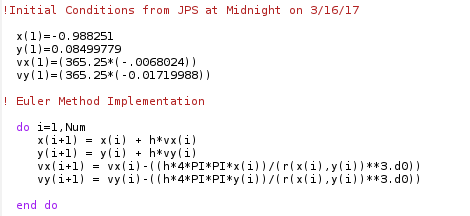
\includegraphics[width=0.8\textwidth]{EulerCode.png}
    \caption{The code used to implement Euler's method for the Sun Earth system.}
\end{figure}

While this algorithm is simple, it is also unstable.  The plot below shows the trajectory of the earth over 10 years in 1000 time steps using initial conditions from the Jet Propulsion Laboratory \cite{JPL} at midnight on March 16,2017.

\begin{figure}[H]\label{fig:eulerplot}
  \centering
    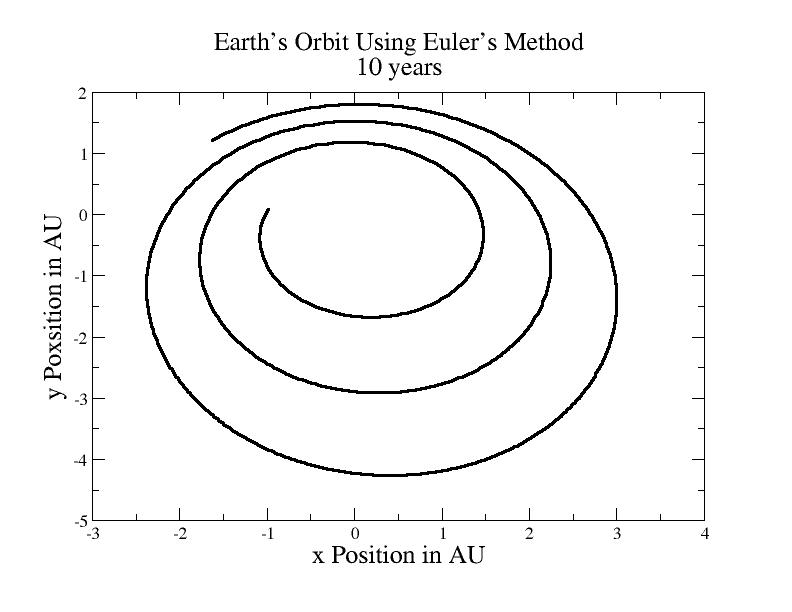
\includegraphics[width=1.0\textwidth]{Euler.jpg}
    \caption{The trajectory of the Earth in the Sun-Earth system produced by Euler's method}
\end{figure}

Almost immediately, the trajectory begins to spin out away from the Sun.  Because of this, there is no point pursuing this method for larger systems.  Instead, we will use the Velocity Verlet method.  The code containing the most important elements of the Velocity Verlet method for the Sun-Earth is shown below.

\begin{figure}[H]\label{fig:velcode}
  \centering
    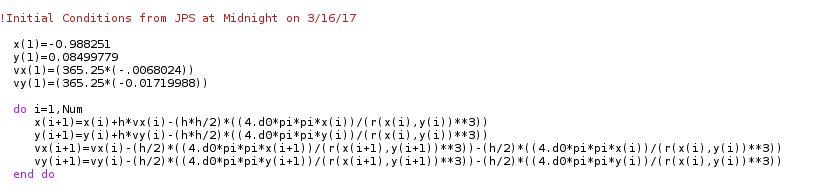
\includegraphics[width=1.0\textwidth]{VelCode.png}
    \caption{The code used to implement the Velocity Verlet method for the Sun Earth system.}
\end{figure}

The plot below shows the trajectory of the earth over 10 years in 1000 time steps using initial conditions from the Jet Propulsion Laboratory at midnight on March 16,2017.

\begin{figure}[H]\label{fig:velrplot}
  \centering
    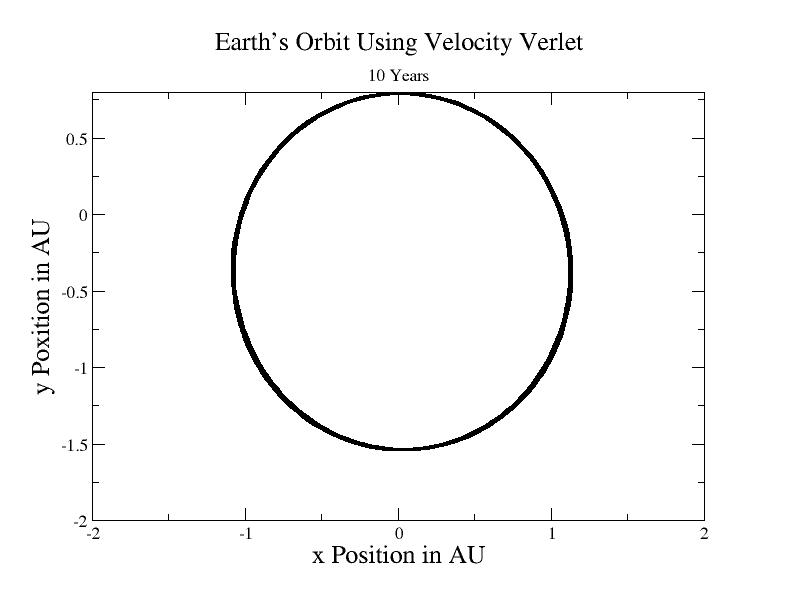
\includegraphics[width=1.0\textwidth]{velverearth.jpg}
    \caption{The trajectory of the Earth in the Sun-Earth system produced by the Velocity Verlet method}
\end{figure}

Unlike Euler's method, the Velocity Verlet algorithm produces a stable, almost circular orbit.  We can investigate to see how much more computationally expensive the Velocity Verlet method is.  If we examine the algorithm for Euler's method and we precalculate as many factors as possible to decrease the number of FLOPS in the main algorithm, Euler's method in two dimensions needs 16N FLOPS where N is the number of time steps taken.  We we apply a similar analysis to the Velocity Verlet algorithm, we get almost 30N FLOPS in 2 dimensions.  

We can also examine this difference by looking at the time it takes to run the algorithm.  Because both methods are very fast, I ran them for the case of 100 years with 100,000 time steps.  This is well above the necessary precision, but will allow for the clocks to accumulate a longer computation time.  The Euler method took 0.3359 seconds to complete that computation, while the Velocity Verlet method required 0.444 seconds.  This shows that the Velocity Verlet algorithm maintains a good balance of precision and computational speed.  Because of this, we will use the Velocity Verlet algorithm to extend our code to the Sun-Earth-Jupiter and Solar systems.  Because all of the equations for this system follow a similar format, we will switch to an OO structure for our code, which will be discussed in more detail in the following section. 

\subsection{Object Oriented Code}

We developed an object oriented version of the Velocity Verlet method to solve the Earth-Sun, Earth-Sun-Jupiter, and Solar systems.  This involved defining a type, which I called "solver" that contained all of the masses, positions, and velocities of the system that you are solving.  This solver also contains a series of subroutines that can be used to calculate relative positions, forces, and recalculate a planet's position, among other things.  This declaration can be seen below.

\begin{figure}[H]\label{fig:velrplot}
  \centering
    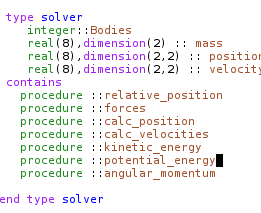
\includegraphics[width=0.5\textwidth]{solver.PNG}
    \caption{Definition of Solver type in OO code.}
\end{figure}

This module is accompanied by a program which makes calls to the procedures in "solver" to apply the Velocity Verlet method.  This program also prints the results to file so they can be plotted.  The heart of this code is shown below.

\begin{figure}[H]\label{fig:velrplot}
  \centering
    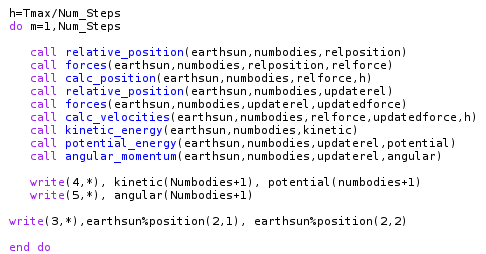
\includegraphics[width=1.0\textwidth]{twobody.PNG}
    \caption{Heart of the main function for the OO program.}
\end{figure}

This portion of the code does not need to be modified at all when the user switches between systems.  All that needs to be changed is the size of arrays in "solver" and  initial conditions.

\subsection{Tests of Code}

There are a number of ways to test the stability of the algorithm.  One thing we can look at is the stability as a function of the step size.  The plot below shows the Earth's orbit with a variety of step sizes.  Each calculation was done for 1 year.  10 steps gives a rough idea of the shape of the orbit.  100 and 1000 steps are nearly indistinguishable.  Because we don't need to do any precision predictions in this report, 100 steps per year is more than sufficient.  It is worth noting, however, that this algorithm is fast, so we could decrease the step size further if we wanted a very precise trace of the orbit.

\begin{figure}[H]\label{fig:velrplot}
  \centering
    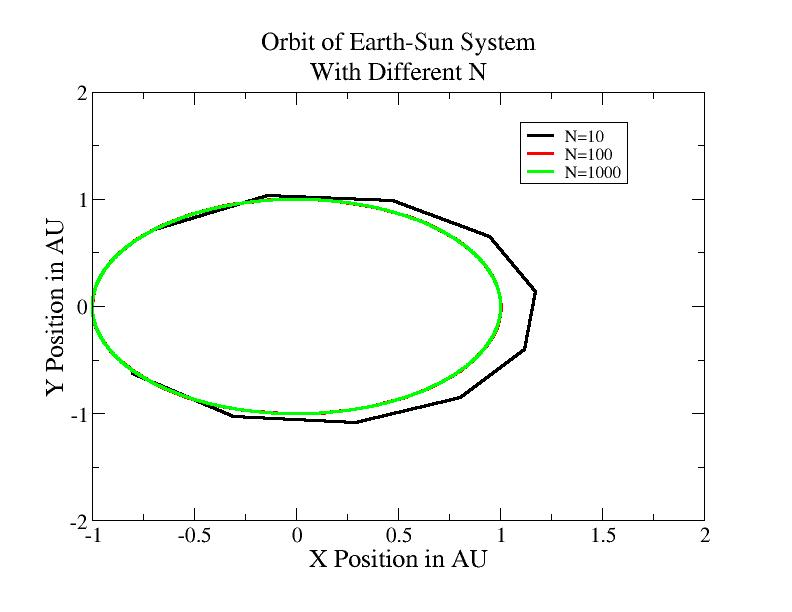
\includegraphics[width=1.0\textwidth]{num.jpg}
    \caption{Plot showing the convergence of the Earth's orbit as a function of the number of time steps.}
\end{figure}

Another thing that we could test is that energy and momentum is conserved.  We know that total energy is always conserved.  In a circular orbit, the magnitude of a planet's velocity and the radius from the center won't change, so this means that potential and kinetic energy should be, individually, conserved.  Additionally, angular momentum will be conserved.  This is easy to test by adding a procedure to the solver type that calculates kinetic energy, potential energy, and angular momentum.  The figures below shows the result of calculating the energy and momentum for the Earth in a circular orbit for 1 year with 100 steps (not all steps shown).  We see that these quantities are, indeed, conserved.  We will discuss the requirements for circular orbit more in the next section.

\begin{figure}[H]\label{fig:velrplot}
  \centering
    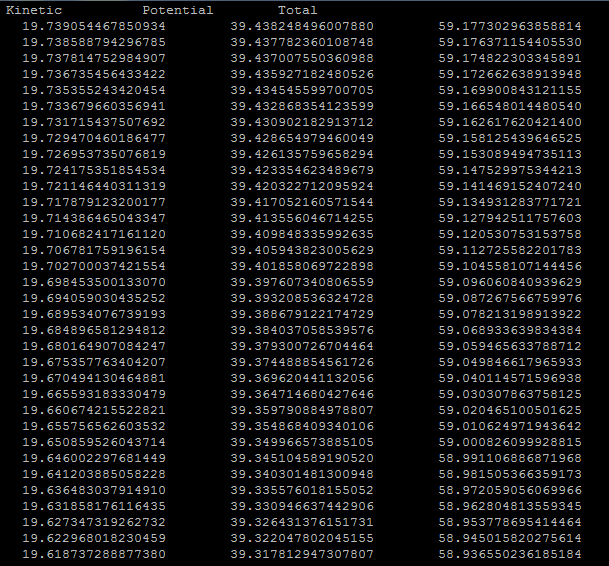
\includegraphics[width=1.0\textwidth]{energy.PNG}
    \caption{Result of energy conservation calculation.  This shows that kinetic and potential energy are independently conserved, as we would expect for a circular orbit.}
\end{figure}

\begin{figure}[H]\label{fig:velrplot}
  \centering
    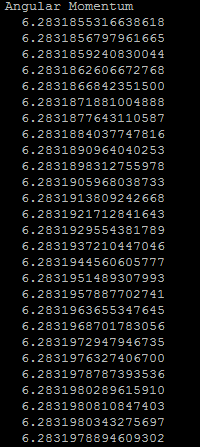
\includegraphics[width=0.3\textwidth]{Momentum.PNG}
    \caption{Result of angular momentum conservation calculation.  This shows that angular momentum is conserved.}
\end{figure}

\section{Results and Discussion}


\subsection{Escape Velocity of the Sun-Earth System}

If an object's kinetic energy exceeds the potential energy keeping it in orbit, it will escape from the system.  This escape velocity can be found by

\[
-\frac{G m_1 M_2}{R}=\frac{1}{2}m_1 v^2
\]
so 
\[
v_{esc}=\sqrt{\frac{2GM_2}{R}}.
\]

The normal orbital velocity can be found by setting the gravitational force equal to the centripetal force.  Solving this leaves us with an orbital velocity of $v_{orb}=\sqrt{\frac{GM_2}{R}}$ so that

\[
v_{escape}=\sqrt{2}v_{orbit}.
\]

For the Earth, the velocity is $2 \pi$ AU/year, so the escape velocity should be roughly $\sqrt{2}2\pi$ AU/year.  The orbital velocity should result in a circular orbit, while increasing the velocity will lead to a more and more ellipsoidal orbit, until the escape velocity is reached and the orbit is broken.  The plot below shows Earth's orbit with a variety of initial velocities.  As we expect, an initial velocity of $2 \pi$ gives a very circular orbit and as we approach $\sqrt{2}2\pi$, the orbit breaks down.

\begin{figure}[H]\label{fig:velrplot}
  \centering
    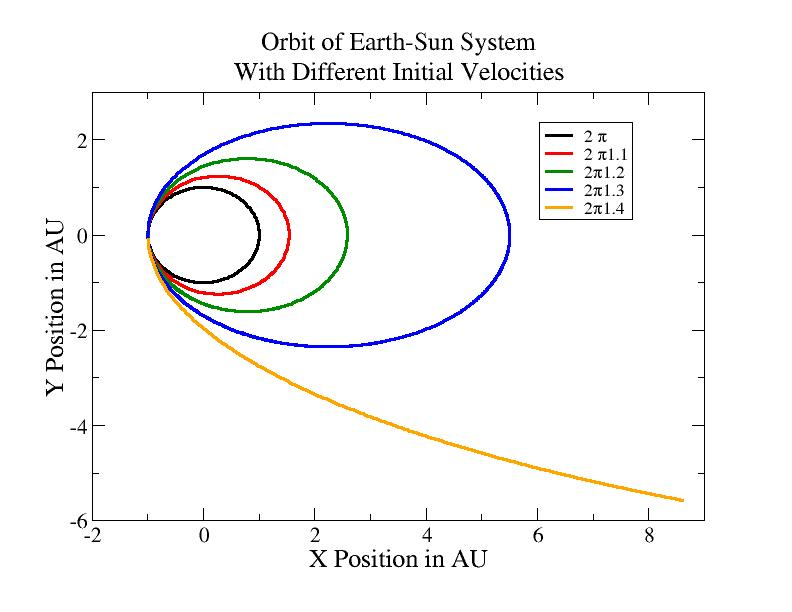
\includegraphics[width=1.1\textwidth]{escape.jpg}
    \caption{Probing the escape velocity of the Earth-Sun system}
\end{figure}

\subsection{The Three Body Problem}

As I mentioned before, the code can be very easily modified to include larger systems.  Here I look at the three body Earth-Sun-Jupiter system.  This subset of planets was chosen because Jupiter is the largest planet in the Solar system, just 1000 times smaller than the sun.  Below is a plot which shows the orbit the this system.  The initial conditions for this orbit come from \cite{JPL} and are the conditions from March 16, 2017.  Although it is difficult to see here, the addition of Jupiter adds small variations to Earth's stable orbit.

\begin{figure}[H]\label{fig:velrplot}
  \centering
    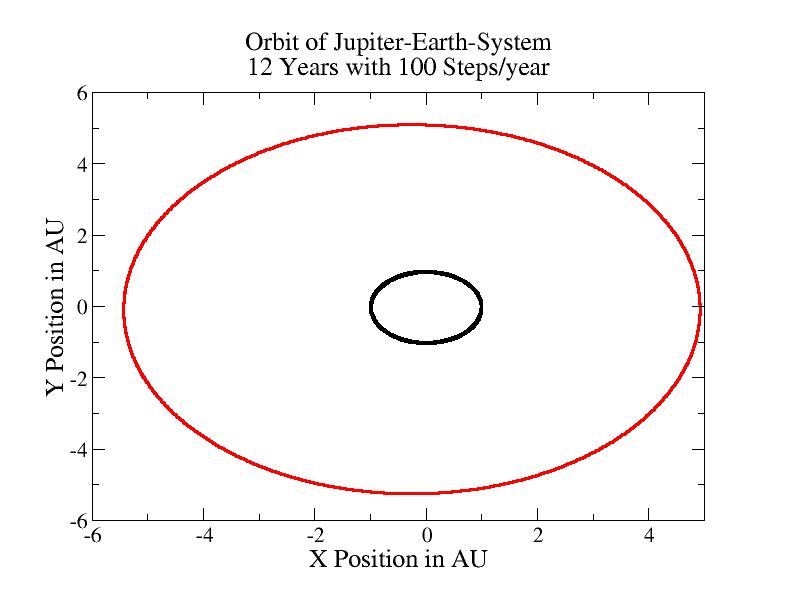
\includegraphics[width=1.1\textwidth]{JESOrbit.jpg}
    \caption{Plot of the Earth-Sun-Jupiter system.}
\end{figure}

Similar to before, we can test the stability of the calculation as a function of step size.  The plot for this gets a little busy, so the results of this stability study are given in the table below.  Note that the period for Jupiter's orbit is 12 years.

\begin{center} 
\begin{tabular}{ |c|c|c| }
\hline
Maximum Time & Number of Steps & Notes \\
\hline
12& 10 & Cannot produce Jupiter's orbit \\
12 & 50 & Cannot produce Jupiter's orbit \\
12 & 75 & Stable orbit for the Earth and Jupiter \\
12 & 1200 & Smooth orbit for Earth and Jupiter \\
12 & 12000 & Can begin to see small variations in Jupiter's orbit\\
\hline
\end{tabular}
\label{table:test}
\end{center}

Another investigation we can do is to explore how the orbit changes if the mass of Jupiter is increased by a factor of 10 or 100.  Those results are shown in the figures below.  In both cases, the orbits become unstable.  Both plots show the evolution over 120 years, or 10 of Jupiter's orbits.

\begin{figure}[H]\label{fig:velrplot}
  \centering
    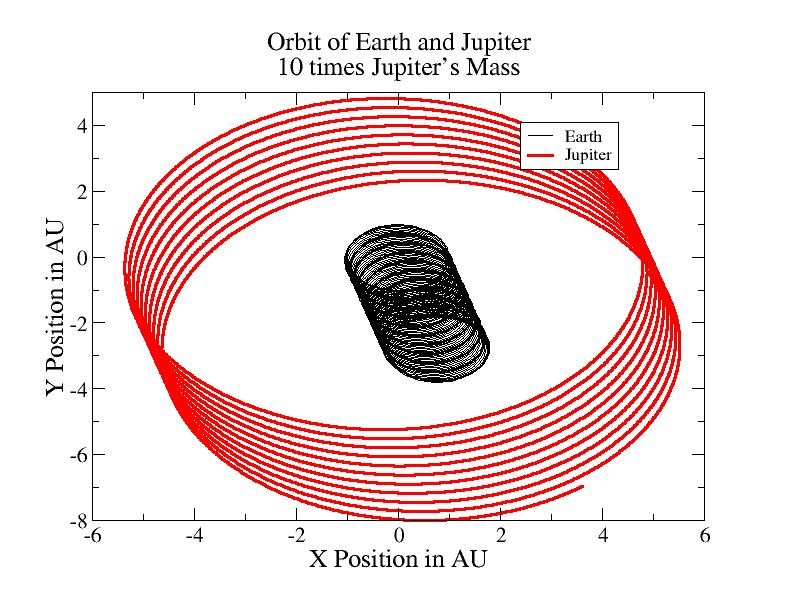
\includegraphics[width=0.85\textwidth]{tenplot.jpg}
    \caption{Plot of the Earth-Sun-Jupiter system with the mass increased by a factor of 10.}
\end{figure}

\begin{figure}[H]\label{fig:velrplot}
  \centering
    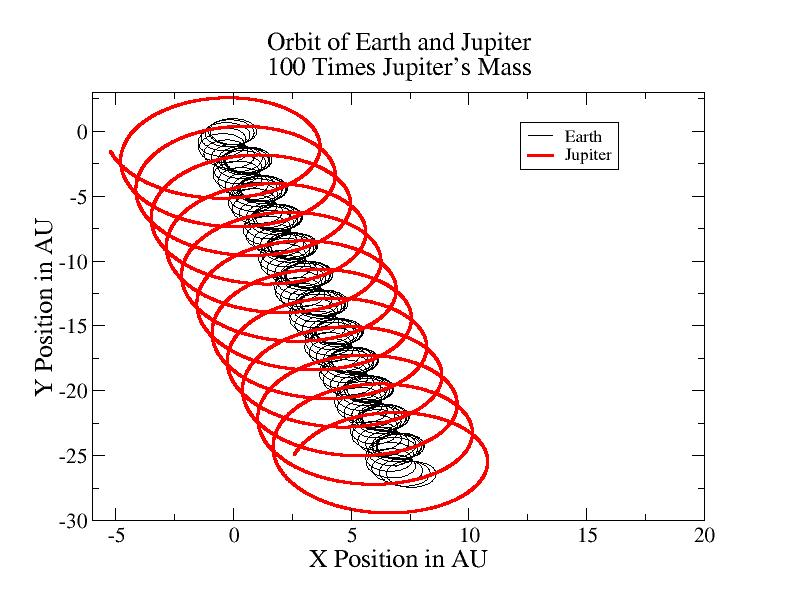
\includegraphics[width=0.85\textwidth]{Jupiter100.jpg}
    \caption{Plot of the Earth-Sun-Jupiter system with the mass increased by a factor or 100.}
\end{figure}

\subsection{Solar System Model}

The next extension is to include the entire Solar System.  Although Pluto is no longer classified as a planet, I included it in this calculation for historical reasons.  Again, the OO format of this code makes for an easy transition between systems.  All of the initial conditions for these calculations come from \cite{JPL} and reflect conditions in the Solar system on March 16, 2017.  For this system, I modified the code to run in three dimensions. In this calculation the Sun is given an initial, non-zero position and velocity.  A plot of the entire Solar system over the course of 250 years (the period of Pluto's orbit) is shown below.  Because there is a large difference in scale between the orbits, I have also plotted the orbit of just the four inner planets. 

\begin{figure}[H]\label{fig:velrplot}
  \centering
    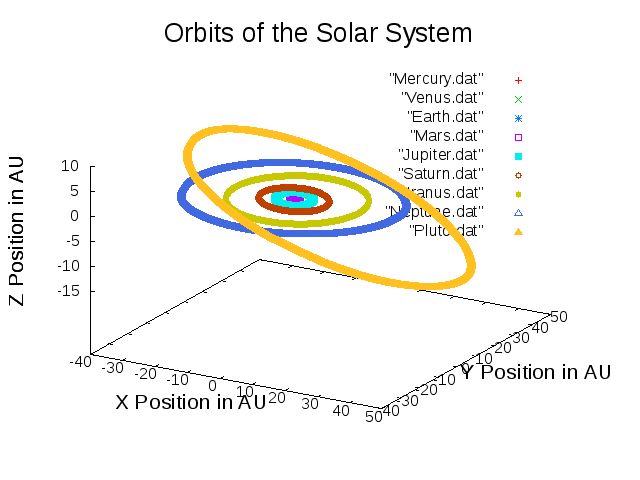
\includegraphics[width=0.85\textwidth]{solarsystem.png}
    \caption{Plot of the Solar system orbits in 3 dimensions}
\end{figure}


\begin{figure}[H]\label{fig:velrplot}
  \centering
    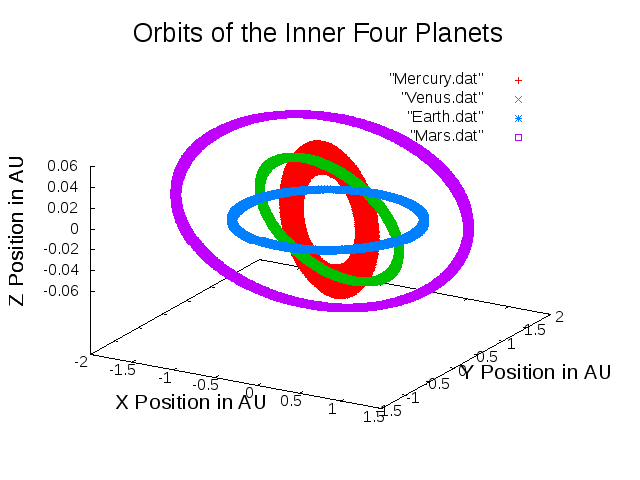
\includegraphics[width=0.85\textwidth]{innersolarsystem.png}
    \caption{Plot of orbits of the four inner planets in 3 dimensions}
\end{figure}

Examining these plots shows us that, other than Pluto, the orbits of the planets are nearly coplanar.  In the plot of the four inner planets, the small scale of the z axis makes it appear otherwise, but upon closer inspections, one sees that variations in the z axis are more than an order of magnitude smaller than in the orbital plane.  Additionally, we can see that Pluto's orbit cuts across Neptune's orbit, just as we would expect from observation.  This is result is also quite comforting because it shows that for the next 250 years (longer than my lifetime) the Solar system should remain stable.  

\section{Conclusions}

In this project, I developed an Object Oriented code the implements the Velocity Verlet method to solve for the evolution of the Solar system under the influence of gravity.  We found this method to be both computationally efficient and precise.  In the Earth-Sun system, our calculations were able to reproduce a $\sqrt{2}2 \pi$ value for the escape velocity of the Earth.  In the three body Sun-Earth-Jupiter system, we saw that the addition of Jupiter added only small variations to the orbit of the Earth. We also found that the system becomes unstable if the mass of Jupiter is greatly increased.  Finally, we looked at the entire solar system and saw that, with the exception of Pluto, the Solar system is nearly coplanar and that the Solar system is stable.

While these results are, themselves, interesting, it is worth noting that this code is powerful because it could be applied to any set of "particles" under the influence of some force.  One would just have to modify the force calculation and the masses to have a code that applies to a new physical system.  This makes Object Oriented programing in which you can "write once, use many times" a powerful tool for scientific computation.

\begin{comment}

\begin{figure}[H]\label{fig:compzoom}
  \centering
    \includegraphics[width=1.2\textwidth]{compzoom.eps}
    \caption{A zoomed in view of the convergence to the exact solution}
\end{figure}

\begin{center} 
\begin{tabular}{ |c|c|c|c| }
\hline
Size of Matrix ($10^n$) & General & Tailored & LU \\
\hline
1& 3.00 E -6 & 3.00 E -6 & 2.40 E -5\\ 
2 & 4.00 E -6 & 4.00 E -6 & 1.71 E -3 \\ 
3 & 3.90 E -5 & 1.90 E -5 & 1.93\\ 
4 & 3.79 E -4 & 2.09 E -4 & N/A\\ 
5 & 3.38 E -3 & 1.51 E -3  & N/A\\ 
6 & 2.87 E -2 & 1.53 E -2 & N/A\\ 
7 & 3.16 E -1 & 1.73 E -1& N/A\\ 
\hline
\end{tabular}
\label{table:test}
\end{center}

\end{comment}

\begin{thebibliography}{9}

\bibitem{LectureNotes} 
Hjorth-Jensen, Mortehn. 
Computational Physics, Lecture Notes Fall 2015. 
August 2015.

\bibitem{JPL} 
Jet Propulsion Laboratory .
HORIZONS Web-Interface. 
http://ssd.jpl.nasa.gov/horizons.cgi.


\end{thebibliography}



% ------------------- end of main content ---------------

\end{document}

